\documentclass{article}

\usepackage{graphicx}
\usepackage{multirow}
\usepackage{siunitx}
\usepackage[table]{xcolor}
\sisetup{
	round-mode= places,
	round-precision= 2,
}

\title{Logic gates}
\author{Anameti Zion Umoh}
\date{13th November 2021.}

\begin{document}
	\pagenumbering{Gobble}
	\maketitle
	\pagenumbering{arabic}
	\newpage
	
	
	Table of Content
	\section{Logic Gates}
	\section{Types of Gates}
	\subsection{AND Gates}
	\subsection{OR Gates}
	\subsection{NAND Gates}
	\subsection{NOR Gates}
	\subsection{XNOR Gates}
	\subsection{XOR Gates}
	
	\newpage
	
	\section{Introduction}
A logic gate is a building block of a digital circuit which is at the heart of any computer operation. \textbf{Behind every digital system is a logic gate.}

\section{Logic Gates}
Logic gates perform logical operations that take binary input (o's and 1s) and produce a single binary output. They are used in most electronic device including:
\begin{table}[h!]
	\begin{center}
		\caption{Logic Gates}
		\label{tab:table1}
		\begin{tabular}{l c c}
			Smartphones
			&
			Tablets
			&
			Memory Devices
			\\
			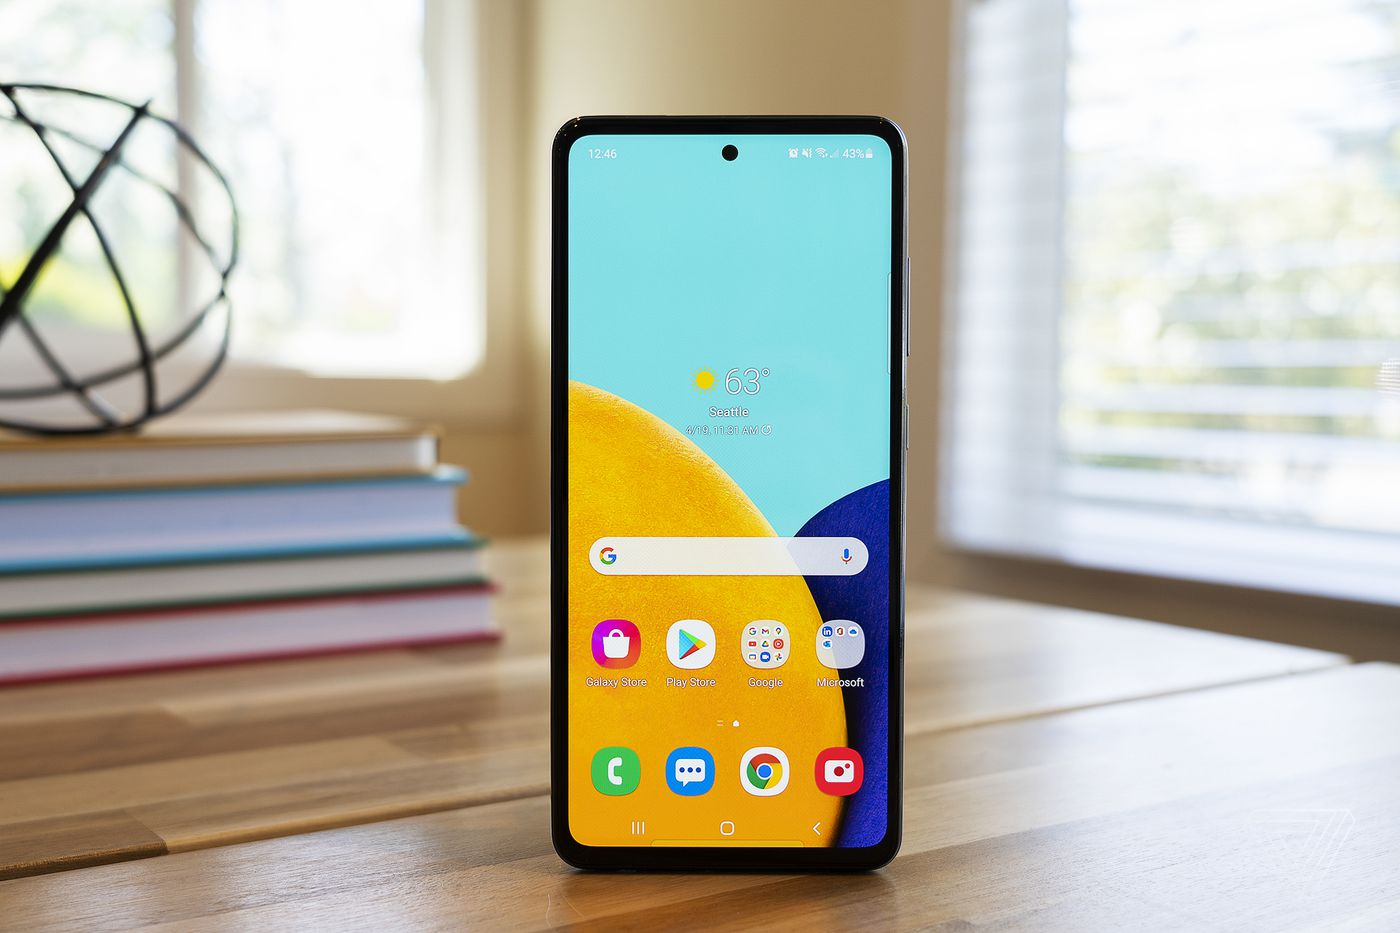
\includegraphics[width=0.2\linewidth]{Picture2}
			&
			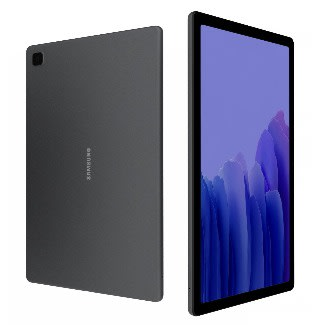
\includegraphics[width=0.25\linewidth]{Picture3}
			&
			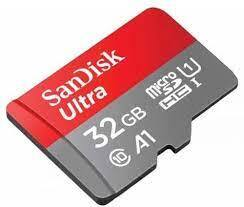
\includegraphics[width=0.2\linewidth]{Picture4}
			\\
		\end{tabular}
	\end{center}
\end{table}

\paragraph{}
Now think of a logic gate like a light switch, it is either in an ON or OFF position. Similarly, the input output terminals are always in one of two binary positions false(0) and true(1). Each gate has its own logic or set of rules that determines how it acts based on multiple inputs outlined in a truth table.
\paragraph{}
Combining 10s, 1000s or millions of logic gates makes it possible for a computer to perform highly complex operations and tasks at ever increasing speeds.

\paragraph{}
A gate is a basic electronic circuit which operates on one or more signals to produce an output signal. 
Logic gates are digital circuits constructed from diodes, transistors, and resistors connected in such a way that the circuit output is the result of a basic logic operation (OR, AND, NOT) performed on the inputs.
\newpage
\section{Types of Logic Gates}
\paragraph{}
Fundamental gates are \textcolor{red}{AND}, \textcolor{red}{OR} and \textcolor{red}{NOT}

\includegraphics[width=1.0\linewidth]{Logicpic}

\paragraph{}
Derived Gates are NAND, NOR, XOR and XNOR (derived from the fundamental gates)
\paragraph{}
Universal Gates are NAND and NOR gates (the fundamental logic gates can be realized through them).

\subsection{AND Gate}
\paragraph{}
The expression C = A X B reads as “C equals A AND B“ 
The multiplication sign (X) stands for the AND operation, same for ordinary multiplication of 1s and 0s.
\begin{table}[h!]
	\begin{center}
		\caption{Logic Gates}
		\label{tab:table1}
		\begin{tabular}{l c c}
			\textcolor{red}{Input}
			&
			\includegraphics[width=0.25\linewidth]{Logicpic2}
			&
			\textcolor{red}{Output}
			\\
		\end{tabular}
	\end{center}
\end{table}
The AND operation produces a true output (result of 1) only for the single case when all of the input variables are 1 and a false output (result of 0) where one or more inputs are 0.
\\
\begin{table}[h!]
	\begin{center}
		\begin{tabular}{ |l|c|c| }
			\cellcolor{blue!100}\textcolor{white}{\textbf{    A    }} & \cellcolor{blue!100}\textcolor{white}{\textbf{    B    }} & \cellcolor{blue!100}\textcolor{white}{\textbf{C=A X B}}\\
			\hline
			1 & 1 & 1\\
			1 & 0 & 0\\
			0 & 1 & 0\\
			0 & 0 & 0\\
			\hline
	
		\end{tabular}
	\end{center}
\end{table}
\section{AND Gate}
\begin{center}
	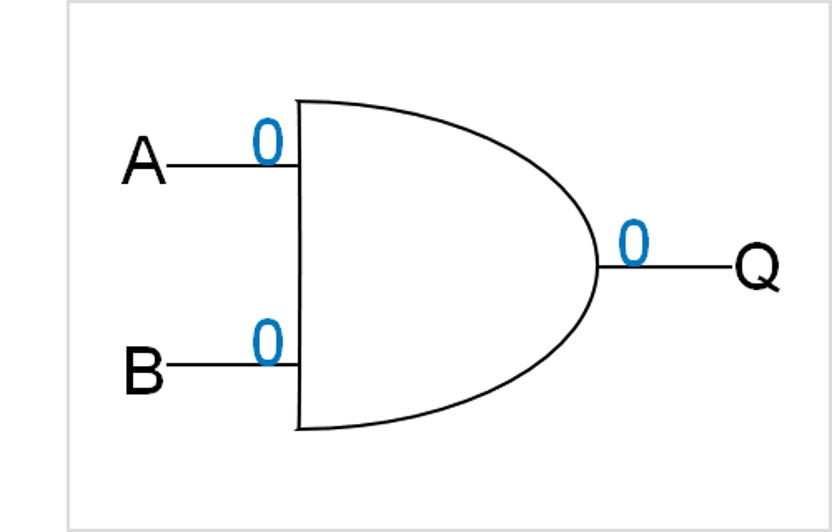
\includegraphics[width=1.2\linewidth]{and}
\end{center}

\section{NOT Gate}
The NOT gate is called a logical inverter.
It has only one input. It reverses the original input (A) to give an inverted output C.
\\
\begin{center}
	\textcolor{red}{\textbf{C = NOT A or C = ~A}}
\end{center}
\begin{table}[h!]
	\begin{center}
		\caption{Logic Gates}
		\label{tab:table1}
		\begin{tabular}{l c c}
			\textcolor{red}{Input}
			&
			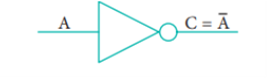
\includegraphics[width=0.25\linewidth]{Logicpic3}
			&
			\textcolor{red}{Output}
			\\
		\end{tabular}
	\end{center}
\end{table}
\\
\begin{table}[h!]
	\label{tab:table1}
	\begin{center}
		\begin{tabular}{ |l|c|c| }
			\cellcolor{blue!100}\textcolor{white}{\textbf{    A    }} & \cellcolor{blue!100}\textcolor{white}{\textbf{C=~A}}\\
			\hline
			1 & 0\\
			0 & 1\\
			\hline
			
		\end{tabular}
	\end{center}
\end{table}
\newpage
\section{NOT Gate}
\begin{center}
	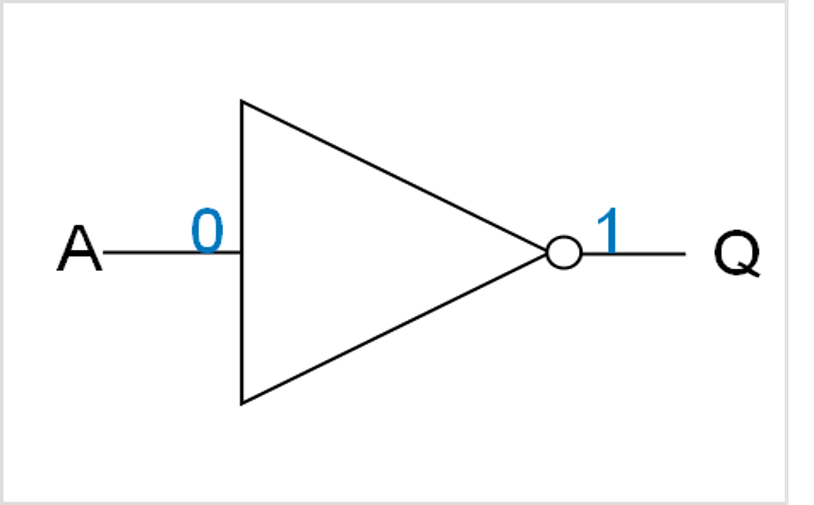
\includegraphics[width=1.2\linewidth]{Not}
\end{center}
\section{NOR Gate}
\paragraph{}
The NOR (NOT OR) gate circuit is an inverter OR gate.
\begin{center}
	C=(~A+~B)
\end{center}
\paragraph{}
Reads as C = NOT of A or B
\\
\paragraph{}
The NOR Gate gives a true output (result of 1) only when both inputs are false (0)
\newpage
\begin{table}[h!]
	\begin{center}
		\caption{Logic Gates}
		\label{tab:table1}
		\begin{tabular}{l c c}
			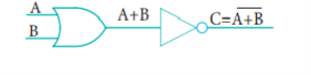
\includegraphics[width=0.25\linewidth]{nor1}
			&
			
\includegraphics[width=0.13\linewidth]{arrow}
			&
			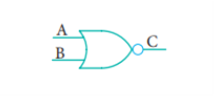
\includegraphics[width=0.25\linewidth]{nor2}
			\\
		\end{tabular}
	\end{center}
\end{table}

\begin{table}[h!]
	\begin{center}
		\begin{tabular}{ |l|c|c|c }
			\cellcolor{blue!100}\textcolor{white}{\textbf{    A    }} & \cellcolor{blue!100}\textcolor{white}{\textbf{    B    }} & \cellcolor{blue!100}\textcolor{white}{\textbf{A + B}} &
			\cellcolor{blue!100}\textcolor{white}{\textbf{C=(A + B)}}\\
			\hline
			1 & 1 & 1 & 0\\
			0 & 0 & 1 & 0\\
			0 & 1 & 1 & 0\\
			0 & 0 & 0 & 1\\
			\hline
			
		\end{tabular}
	\end{center}
\end{table}
\paragraph{}
\textcolor{red}{\textbf{The NOR Gate is a universal gate because it can be used to form any other kind of gate }}
\section{NOR Gate}
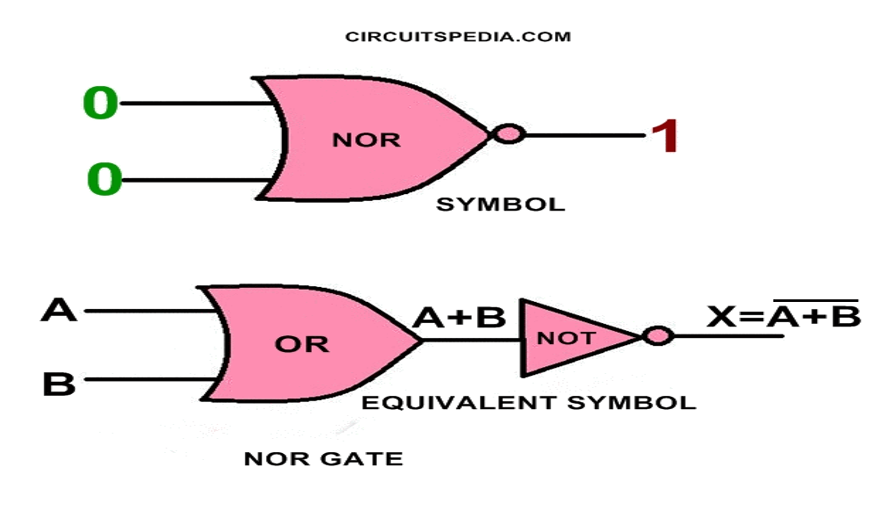
\includegraphics[width=1.2\linewidth]{norm}

\section{NAND Gate}
\paragraph{}
The NAND (NOT AND) Gate is an inverted AND Gate

\begin{center}
	C=(~Ax~B)
\end{center}
\paragraph{}
Reads as C = NOT of A AND B
\\
\paragraph{}
The NAND Gate gives a false output (result of 0) only when both inputs are true (1)
\newpage
\begin{table}[h!]
	\begin{center}
		\caption{Logic Gates}
		\label{tab:table1}
		\begin{tabular}{l c c}
			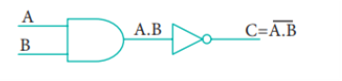
\includegraphics[width=0.25\linewidth]{nand1}
			&
			
\includegraphics[width=0.13\linewidth]{arrow}
			&
			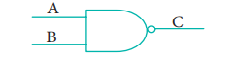
\includegraphics[width=0.25\linewidth]{nand2}
			\\
		\end{tabular}
	\end{center}
\end{table}

\begin{table}[h!]
	\begin{center}
		\begin{tabular}{ |l|c|c|c }
			\cellcolor{blue!100}\textcolor{white}{\textbf{    A    }} & \cellcolor{blue!100}\textcolor{white}{\textbf{    B    }} & \cellcolor{blue!100}\textcolor{white}{\textbf{A + B}} &
			\cellcolor{blue!100}\textcolor{white}{\textbf{C=(A + B)}}\\
			\hline
			1 & 1 & 1 & 0\\
			1 & 0 & 0 & 1\\
			0 & 1 & 0 & 1\\
			0 & 0 & 0 & 1\\
			\hline
			
		\end{tabular}
	\end{center}
\end{table}
\paragraph{}
\textcolor{red}{The NAND Gate is a universal gate because it can be used to form any other kind of gate }
\section{NOR Gate}
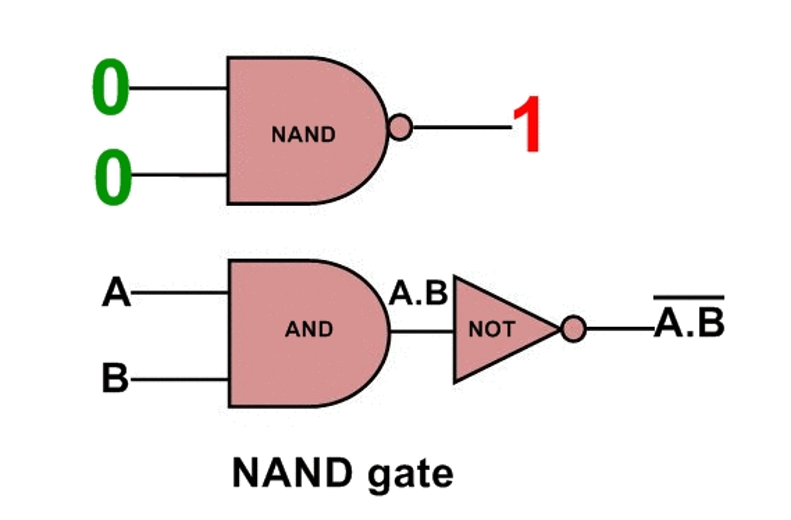
\includegraphics[width=1.2\linewidth]{nandm}
\newpage



\section{XOR Gate}
\paragraph{}
An XOR (exclusive OR) gate acts in the same way as the exclusive OR logical connector. 
\paragraph{}
It gives a true output (result of 1) if one, and only one, of the inputs to the gate is true (1), i.e either or but not both.
\begin{center}
	C = A ~+ B = ~A.B + ~B.A
\end{center}
\\
\begin{table}[h!]
	\begin{center}
		\caption{Logic Gates}
		\label{tab:table1}
		\begin{tabular}{l c c}
			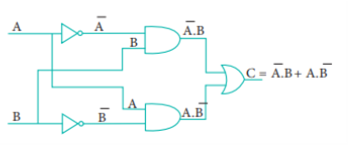
\includegraphics[width=0.25\linewidth]{xor1}
			&
			
\includegraphics[width=0.13\linewidth]{arrow}
			&
			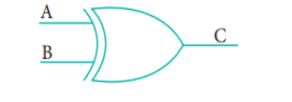
\includegraphics[width=0.25\linewidth]{xor2}
			\\
		\end{tabular}
	\end{center}
\end{table}

\begin{table}[h!]
	\begin{center}
		\begin{tabular}{ |l|c|c|c|r|r|r| }
			\cellcolor{blue!100}\textcolor{white}{\textbf{    A    }} & 
			\cellcolor{blue!100}\textcolor{white}{\textbf{    B    }} & \cellcolor{blue!100}\textcolor{white}{\textbf{~A}} &
			\cellcolor{blue!100}\textcolor{white}{\textbf{~B}} &
			\cellcolor{blue!100}\textcolor{white}{\textbf{~A.B}} &
			\cellcolor{blue!100}\textcolor{white}{\textbf{~B.A}} &
			\cellcolor{blue!100}\textcolor{white}{\textbf{~A.B + ~B.A}}\\
			\hline
			1 & 0 & 0 & 0 & 0 & 0 & 0\\
			1 & 0 & 0 & 1 & 0 & 1 & 1\\
			0 & 1 & 1 & 0 & 1 & 0 & 1\\
			0 & 0 & 1 & 1 & 0 & 0 & 0\\
			\hline
			
		\end{tabular}
	\end{center}
\end{table}
\newpage
\section{XNOR}
\paragraph{}
The XNOR (exclusive - NOR) gate is a combination XOR gate followed by an inverter. It is represented by the ⊙
\paragraph{}
Its gives a  true output (1), if the inputs are the same, and a false output (0) if the inputs are different. 
\begin{center}
	C = ~A + ~B = ~A.B + ~B.A
\end{center}


\begin{table}[h!]
	\begin{center}
		\caption{Logic Gates}
		\label{tab:table1}
		\begin{tabular}{l c c}
			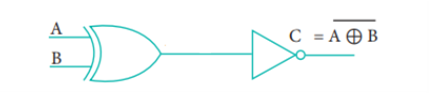
\includegraphics[width=0.25\linewidth]{xnor}
			&
			
\includegraphics[width=0.13\linewidth]{arrow}
			&
			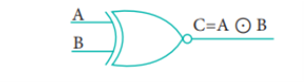
\includegraphics[width=0.25\linewidth]{xnor1}
			\\
		\end{tabular}
	\end{center}
\end{table}
\\
\begin{table}[h!]
	\begin{center}
		\begin{tabular}{ |c|c|c|c|c|c|c|c|}
			\cellcolor{blue!100}\textcolor{white}{\textbf{A}} & \cellcolor{blue!100}\textcolor{white}{\textbf{B}} & \cellcolor{blue!100}\textcolor{white}{\textbf{~A}} &
			\cellcolor{blue!100}\textcolor{white}{\textbf{~B}} &
			\cellcolor{blue!100}\textcolor{white}{\textbf{~A.B}} &
			\cellcolor{blue!100}\textcolor{white}{\textbf{~B.A}} &
			\cellcolor{blue!100}\textcolor{white}{\textbf{~A.B + ~B.A}} &
			\cellcolor{blue!100}\textcolor{white}{\textbf{~(~A.B + ~B.A)}}\\
			\hline
			1 & 1 & 0 & 0 & 0 & 0 & 1 & 1\\
			1 & 0 & 0 & 1 & 0 & 1 & 1 & 0\\
			0 & 1 & 1 & 0 & 1 & 0 & 1 & 0\\
			0 & 0 & 1 & 1 & 0 & 0 & 0 & 1\\
			\hline
			
		\end{tabular}
	\end{center}
\end{table}
\section{Logic Gates and their Truth Tables}
\begin{center}
	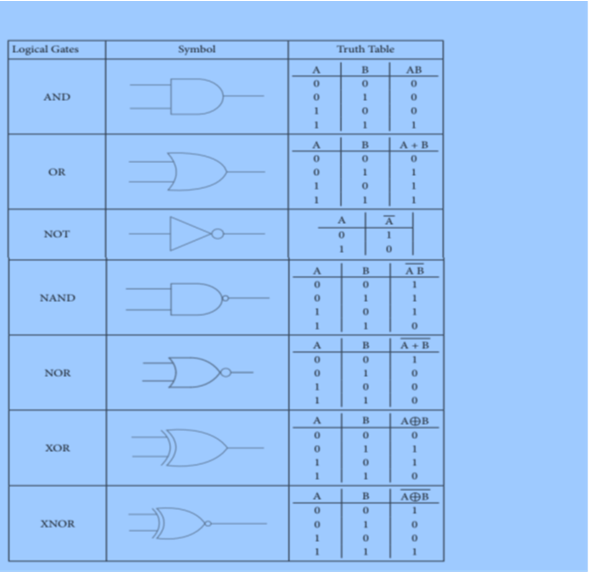
\includegraphics[width=0.5\linewidth]{logictable}
\end{center}
\newpage
\section{Summary}
\paragraph{}
Using different combination of logic gates, complex operations can be performed. 
With the Universal logic gates - NAND and NOR, any other gate can be built
There is no limit to the number of gates that can be arranged together in a single device.
\paragraph{}
However, in practice, there is a limit to the number of gates that can be packed into a given physical space. 
Arrays of logic gates are found in digital integrated circuits.
\paragraph{}
The logic gates are abstract representations of real electronic circuits
In computers, Logic gates are built using transistors combined with other electrical components like resistors and diodes. 
These electrical components are wired together in order to transform a particular input to give a desired output.

\newpage
\begin{center}
	\section{\textbf{QUIZ}}
\end{center}
\paragraph{}
What is the output of an AND gate if the inputs are 1 and 0?
Explain the difference between the AND gate and the OR gate.
\paragraph{}
What is the output of a NOT gate if the inputs is 0?
Which logic gate is this?
Which gate is also known 
a logical converter?
\begin{figure}[h!]
	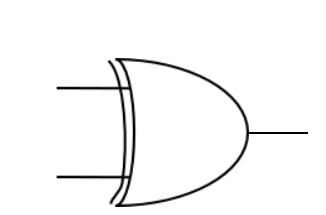
\includegraphics[width=.6\textwidth,left]{quiz}
\end{figure}
\end{document}	